\section{Infrastruttura di rete}
Avere un'infrastruttura di rete progettata in maniera efficace è di \textbf{fondamentale importanza}, tutte le operazioni quotidiane dipendono da essa. Quando si progetta un'infrastruttura non bisogna soltanto considerare la topologia di rete; è necessario infatti tenere conto anche di:
\begin{itemize}
    \item \textbf{dispositivi hardware}: server, datacenter, personal computer, router, switch; è importante fare delle scelte adatte e mirate al caso d'uso.
    \item \textbf{applicazioni e software}: applicazioni utilizzate dall'azienda, come web server, sistemi di gestione del contenuto e sistema operativo, ad esempio Linux. 
\end{itemize}

% \begin{itemize}
%     \item \textbf{Hardware}: include server, datacenter, personal computer, router, switch e altre dotazioni.
%     È da considerare parte dell'infrastruttura anche le strutture che ospitano il datacenter o che forniscono i sistemi di raffreddamento o alimentazione.
%     \item \textbf{Software}: si fa riferimento alle applicazioni utilizzate dall'azienda, come web server, sistemi di gestione del contenuto e sistema operativo, ad esempio Linux. Il sistema operativo gestisce le risorse di sistema e l'hardware e stabilisce inoltre tutte le connessioni necessarie fra i vari componenti software e le risorse fisiche che svolgono le operazioni.
%     \item \textbf{Rete}: l'interconnessione tra i componenti di rete consente l'esecuzione delle operazioni di rete, la gestione e la comunicazione tra i sistemi interni ed esterni. Per il funzionamento di una rete sono indispensabili la connessione a Internet, gli strumenti di attivazione, il firewall e la sicurezza, nonché l'hardware, ovvero router, switch e cavi
% \end{itemize}

Quali sono invece alcuni aspetti da considerare? 
\begin{itemize}
    \item \textbf{Efficienza}: creare un'infrastruttura di rete efficiente riduce al minimo i tempi di down e assicura la stabilità della rete.
    \item \textbf{Scalabilità}: una solida infrastruttura di rete supporta la crescita senza doverla riprogettare.
    \item \textbf{Sicurezza}: deve fornire sicurezza e protezione da spam, malware e virus. Deve anche mantenere i dati al sicuro.
    \item \textbf{Portata}: deve permettere agli utenti di essere connessi alla rete, indipendentemente dalla loro posizione.
\end{itemize}


% \subsection{Analisi dei requisiti}

% Tenendo a mente questi aspetti è ora possibile procedere con l'analisi della richiesta. Sarà necessario:
% \begin{itemize}
%     \item Hardware: fare delle scelte precise e mirate riguardo i \textbf{dispositivi} e le loro caratteristiche tecniche
%     \item predisporre un server che fornisce localmente a tutti i dispositivi collegati dei servizi usati dall'applicazione mobile scaricata dai visitatori. Questo server deve inoltre gestire il pannello di amministrazione.
%     \item progettare una \textbf{topologia di rete} con:
%       \begin{itemize}
%           \item una rete amministrativa per i computer gestionali. È necessario assicurarsi che soltanto i dispositivi di questa sottorete possono accedere al pannello di amministrazione e ad internet
%           \item una rete accessibile a tutti, che permette ai visitatori di connettersi da ogni parte del museo in modo \textbf{wireless}, assicurandosi che i dispositivi collegati al \textbf{Wi-Fi} non abbiano accesso a internet e al pannello di amministrazione
%           \item un \textbf{server} configurato in modo sicuro, accessibile soltanto dalla rete locale, che fornisce le API per far funzionare il client mobile
%       \end{itemize}
% \end{itemize}

\subfile{beacons}

\subsection{Rete}
Il migliore modo per rappresentare la rete nel suo insieme è attraverso una \textbf{topologia}. Essa è una \textbf{mappa} che descrive i dispositivi e come sono collocati. Esistono due tipi di topologie:
\begin{itemize}
    \item \textbf{Topologia fisica}: indica la disposizione fisica dei dispositivi e dei mezzi trasmissivi
    \item \textbf{Topologia logica}: evidenzia il modo in cui gli host accedono al mezzo trasmissivo per inviare dati
\end{itemize}Essendo il luogo non definito, è impossibile realizzare la topologica fisica. Riguardo la topologia logica la maggior parte delle reti wireless utilizza una \textbf{topologia a stella}. Essa consiste in un nodo gateway (in questo caso un \textbf{Access Point}, AP) a cui tutti gli altri nodi si collegano. I vantaggi di questa scelta sono sicuramente:
\begin{itemize}
    \item prestazione della rete veloce e affidabile.
    \item i nodi/dispositivi difettosi possono essere identificati e isolati rapidamente.
\end{itemize}
Mentre gli svantaggi sono: 
\begin{itemize}
    \item la portata è limitata al raggio di trasmissione di un singolo dispositivo.
    \item se il nodo gateway fallisce, l'intera rete smette di funzionare
\end{itemize}
\clearpage
Ai vari dispositivi dei vistatori è necessario aggiungere:
\begin{itemize}
    \item il \textbf{server}
    \item il \textbf{router}
    \item uno o più \textbf{switch}
    \item i vari \textbf{access point} a cui si collegano i dispositivi dei vistatori
\end{itemize}

\begin{center}
    \begin{figure}[htp]
        \centering
        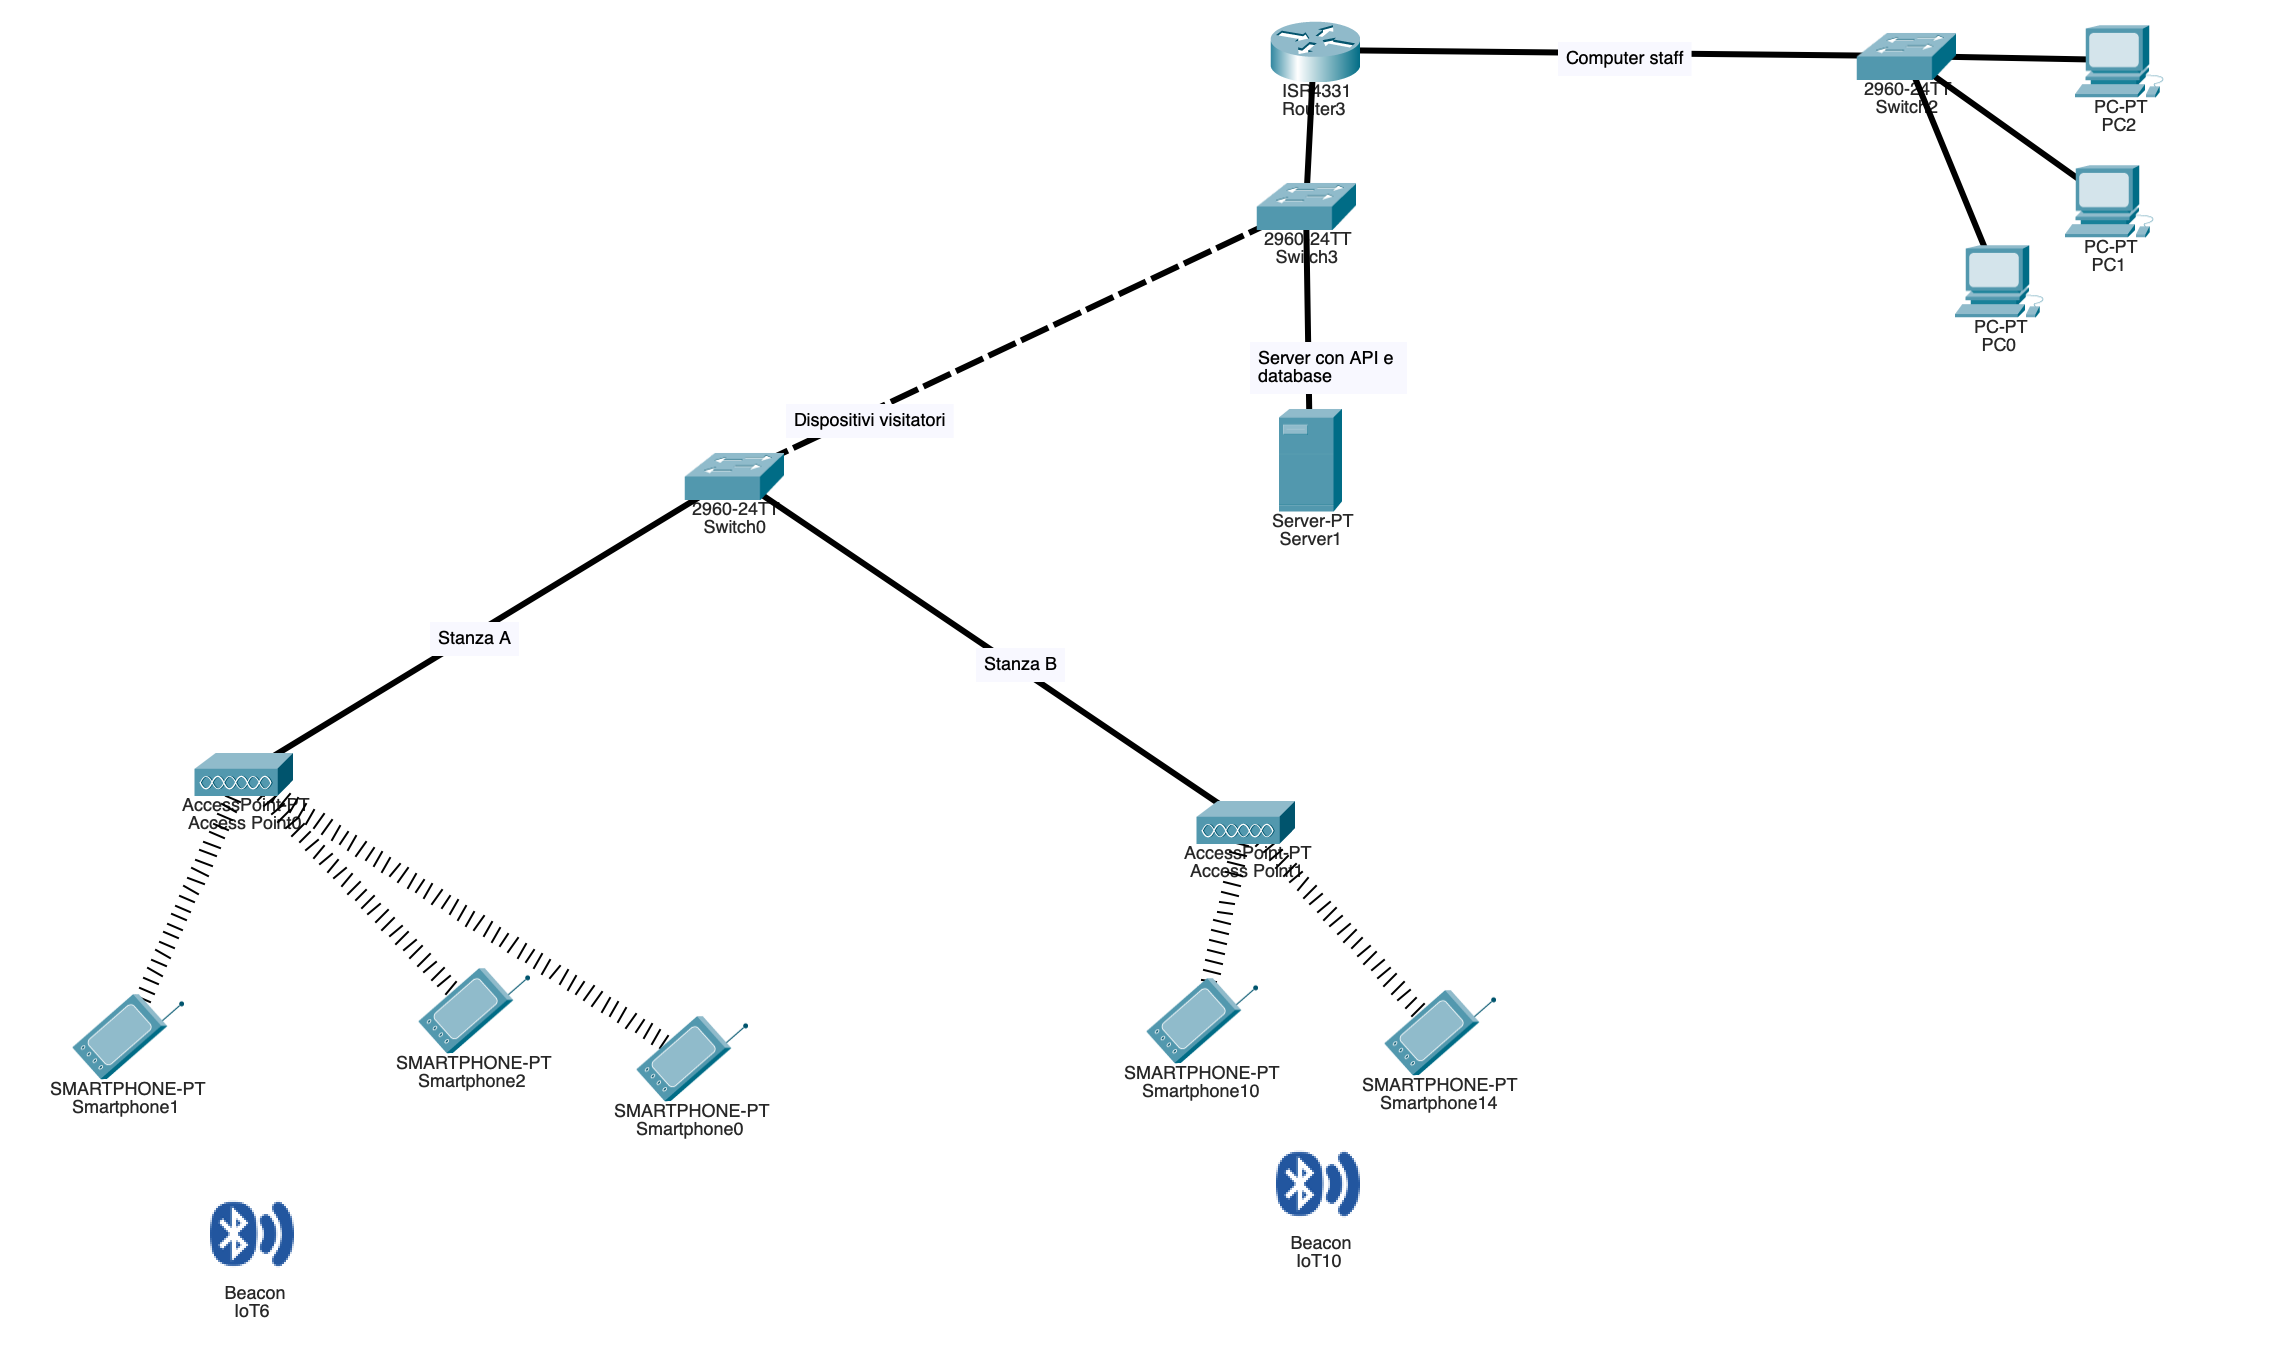
\includegraphics[width=\textwidth]{diagrams/network_diagram_v3.png}
        \caption{Topologia logica}
        \label{fig:topologia_logica}
    \end{figure}
\end{center}

\subsection{Server}
Come server è stata utilizzata una \textbf{virutal machine} con \textbf{Ubuntu Server 21.04}, una distribuzione ufficiale di Ubuntu dedicata all'ambito server. La principale differenza con la distribuzione standard è l'ambiente desktop: mentre Ubuntu Desktop include un'interfaccia grafica utente, Ubuntu Server no. Inoltre la versione server include anche pacchetti standard che si concentrano principalmente sulla connettività e sicurezza.\cite{ubuntu_server_guide}.\\\\Per fornire le API è stato usato \textbf{\href{https://www.nginx.com/}{nginx}}, un web server/reverse proxy leggero ad alte prestazioni. Questa virtual machine è contenuta in un container \textbf{\href{https://www.docker.com/}{Docker}}, un sistema per l'automazione del deployment che considera i container come macchine virtuali modulari estremamente leggere, offrendo la flessibilità di creare, distribuire, copiare e spostare i container da un ambiente all'altro in modo sicuro.\cite{docker_guide}

\clearpage

\subsection{Uso delle API}
L'applicazione non accede direttamente al database, usa delle API. Creare un livello extra di astrazione non è solo utile per la sicurezza, ma anche per la scalabilità. 
\subsubsection{Cosa sono le API}
Un'API, interfaccia di programmazione di un’applicazione, è un insieme di comandi formalizzati che consentono alle applicazioni software di comunicare tra loro in modo uniforme e di sfruttare i servizi di base per creare servizi incentrati sul cliente. Quindi in questo caso il server esegue una applicazione che espone delle API che fanno comunicare il client Flutter con il database MySQL. 

\begin{center}
\begin{figure}[htp]
    \centering
    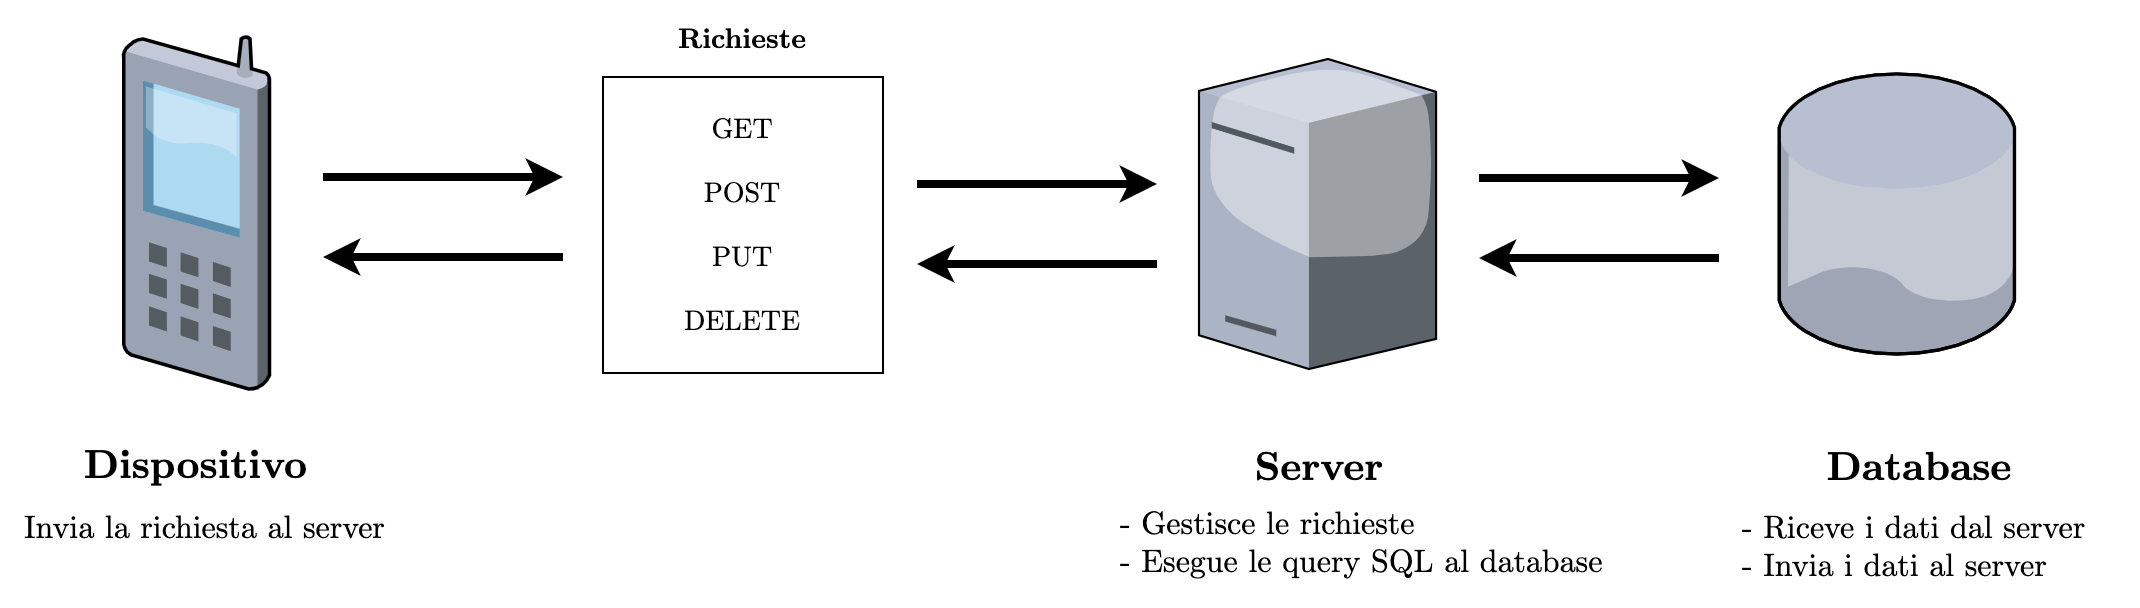
\includegraphics[width=12cm]{diagrams/diagramma_backend.png}
    \caption{L'interazione tra dispositivo, server e database}
    \label{fig:interazione_backend}
\end{figure}
\end{center}


